% ============================================================
%  appendices.tex
%  Appendices A through G
%  COMP3931 Individual Project  Adhiraj Kumar  2025/26
% ============================================================

\begin{appendices}

% ============================================================
\chapter{Self-Appraisal}
\label{app:self_appraisal}
% ============================================================

\section{Critical Self-Evaluation of the Project Process}
\label{sec:self_eval}

The project achieved its goals to an extent, the results and findings were good, which was a relief as I was not always sure it would. A working adaptive drift detection framework was designed, 
implemented, tested across 23 experiments on 50 instruments, and evaluated against 
three research questions. The 121-test suite passes on the committed codebase and all 
results are reproducible from the repository. I am reasonably proud of that. 

The hardest part of this project was not the KS detector, or the calibration logic, 
or the Sharpe decomposition. It was the first three weeks, when I had no idea what the 
project actually was. I knew I wanted to do something in financial machine learning. I remember proposing a couple of different ideas to Dr Chakraborty, and he guided me in the right direction of it being a computer science dissertation first rather than a finance dissertation. Another challenge was I wasn't sure what was rigorous or not rigorous, I kept 
proposing things to myself that were either obviously too thin (one detector, one 
dataset, done) or obviously too large (a live streaming system with real market 
integration that would have taken two years). The version you are reading now, a 
batch-mode adaptive framework across a broad instrument corpus, only existed because 
I eventually forced myself to write down what I was doing in one paragraph and not 
change it afterwards. As Professor Indrusiak guided me in our supervisor meeting, I made sure to try and keep it as a narrative arc and structure and build it up as the report goes along rather than it feeling like stuff being thrown at the reader. 

A related problem was that I confused complexity with quality for longer than I should 
have. My instinct for most of the first half of the project was that more components 
meant a more serious dissertation. The ablation results fixed that. PH alone matched 
the full four-detector ensemble on accuracy delta and ran in half the time. The data 
told me the complexity was not doing anything, and I had to trust that and simplify. 
That was uncomfortable. It felt like admitting the extra work had not paid off. But 
reporting it still felt like a win, and it is one of the findings I am most 
confident in because it went against what I expected.

The phased development structure worked well: data layer, then detectors, then 
controller, then experiments. Committing experiment outputs alongside code at each 
stage meant findings from earlier phases were immediately available rather than 
requiring re-runs. The end-to-end test on AAPL 2018 to 2022 caught several bugs the 
unit tests had missed. These were good decisions. I wish I could say they were planned 
from the start rather than arrived at through trial and error. (As Professor Indrusiak mentioned in the meeting)

The calibration module was not a good decision, or at least not a well-timed one. I 
added it in phase three, after realising that fixed global thresholds produced very 
different false alarm rates across asset classes. This meant revisiting the controller 
design and re-running earlier experiments. If I had read the Basel~II PSI literature 
more carefully at the start, I would have seen this coming. I did not, and I paid for 
it in late nights in February. The position gate was similar: I added it after the 
Sharpe decomposition told me it was contributing 21\% of the Sharpe improvement, more 
than improved directional accuracy alone. Both should have been design 
components from the beginning but they were not, and the project would have been cleaner 
if they had been.

\section{Personal Reflection and Lessons Learned}
\label{sec:reflection}

\paragraph{On not knowing what to do and methodology.}
One of the hardest parts was to figure out what to actually build and do. As Dr Chakraborty would remember in our second meeting where I deeply concerned him with a couple of my ideas not being completely clear or related to Computer Science. His guidance was incredibly valuable in grounding me to a project deeply rooted in Computer Science and also one that I am interested in with the finance component. Another challenge was not knowing when to stop, and not knowing what constitutes as rigorous enough. After being satisfied with the set up, I ran a couple thousand ablation tests to get as much data as I could to see if it works or not, and in the end the results confirmed that the system works to an extent and where it doesn't work, which I documented. 

Some of the parameters felt a bit hard to justify properly, there was always a question of what if? but in the end I decided to stick to the parameters mentioned in the report. I did run multiple tests to see if they're the ideal combination of parameters and was reasonably satisfied with them. For the Composite Drift Index weights, I gave more weightage to the feature signal because it is the earliest signal. It is the only parameter I set without running experiments. 

\paragraph{The look-ahead bug.}
The reference window initialisation error was the most alarming moment of the project. 
The controller was computing the reference window on data that included the first few 
rows of the test period. This introduced look-ahead bias, and the accuracy figures 
looked plausible rather than suspicious, which is the worst possible version of a bug. 
It was caught by the temporal integrity unit test, but only after two preliminary 
experiment runs had produced numbers I was briefly quite pleased with. The lesson, 
which I will not forget, is that look-ahead bias does not announce itself. You have to 
design the tests that catch it before you trust any results at all.

\paragraph{Calibration taking three times as long as expected.}
I budgeted a few days for the calibration module but instead it took the better part of two weeks. 
Instruments with very short reference windows, instruments where the drift index had 
near-zero variance in quiet periods, the fallback logic when calibration could not 
produce reliable limits: each edge case required its own test and its own handling. 
I remember thinking at the time that this kind of thing never shows up in papers, the 
twelve edge cases you have to handle before the elegant method actually works. It does 
not make the papers less useful, but it does make them slightly misleading about what 
implementation actually looks like.

\paragraph{What I would change.}
Calibration module in phase one. End-to-end integration test written before any 
experiment scripts. More time on analysis and less on implementation. The lead-time 
analysis was finished in the final week and ended up reshaping the framing of Chapter~2 
retrospectively. Had I done it earlier, the whole structure would have been cleaner 
from the start. I also would have committed to a scope earlier and protected it more 
aggressively. Scope creep when you are the only person on a project is bad
because there is nobody to tell you to stop. I really appreciate Dr Chakraborty and Professor Indrusiak's advice to know when to stop. 

\paragraph{On supervision a.}
Dr Dibyayan Chakraborty was my supervisor. He was supportive and available, and during 
the periods when the project felt like it was going nowhere, it was very helpful to get his opinion. Meetings 
were encouraging even when they were not technically directive, and there is a version 
of this project that stalled out in November without that. The feedback that changed 
the dissertation most concretely, however, came from my assessor. The recommendation 
to report all 16 ablation configurations rather than a curated subset was the single 
most consequential piece of feedback I received. It forced me to look at the full 
Pareto frontier, which is where the RQ3 finding actually lived: PH alone is 
Pareto-optimal, the lead-time hypothesis is rejected, and a four-detector ensemble 
adds cost without adding value. That is a better finding than what I had planned to 
report, and I would have buried it in a footnote without being pushed to surface it. 
The broader narrative structure of the dissertation, leading with limitations as 
results rather than treating them as qualifications, also came from that conversation. 
It changed how I thought about what honest empirical reporting looks like.


\section{Legal, Social, Ethical and Professional Issues}
\label{sec:lsep}

\subsection{Legal Issues}
\label{subsec:legal}

Price and volume data were sourced from Yahoo Finance via the \texttt{yfinance} library and from FRED via \texttt{fredapi}. Yahoo Finance's terms of service permit use of data for personal and research purposes but prohibit commercial redistribution. The data are used here exclusively for academic research. No raw price data are included in the dissertation or the public repository. FRED data are published by the Federal Reserve Bank of St.\ Louis and are in the public domain.

No personal data about individuals were collected, processed, or stored at any point in the project. The framework operates on aggregated market price and volume data. There are no data subjects, and no obligations arise under the UK General Data Protection Regulation (UK GDPR) or the Data Protection Act 2018.

The framework produces trading signals, but it does not constitute investment advice and is not intended for use as such. The Financial Conduct Authority~\cite{fca2018} defines investment advice as a personal recommendation to buy or sell a specific financial instrument. The framework produces model outputs on historical data. It makes no personal recommendations and has no connection to a live execution system. A disclaimer to this effect is included in the repository README.

MiFID~II~\cite{mifid2014} requirements relevant to the framework's design are discussed where they arise in the methodology, specifically the T+2 settlement cycle justification for the 5-day cooldown. The framework is not subject to MiFID~II as an operational system, as it is a research prototype and not a live trading system.

\subsection{Social Issues}
\label{subsec:social}

Algorithmic trading systems have documented social consequences that are worth considering even for a research prototype. Kirilenko et al.~\cite{kirilenko2017} analyse the 2010 Flash Crash and conclude that high-frequency algorithmic trading contributed to a brief but severe market dislocation, demonstrating that automated trading systems can have systemic effects far exceeding their individual scale. Having worked at a proprietary trading firm myself, it was interesting noting how block trades affect the market dynamics, and while it is not relevant here, it is interesting to note still. 

A framework of the type developed here, if deployed at scale by multiple institutional participants, could contribute to herding behaviour. If many systems detect the same distributional shift and retrain simultaneously, their correlated trading responses could amplify rather than dampen the regime transition. This procyclical dynamic is an acknowledged risk in the algorithmic trading literature~\cite{kirilenko2017,pasquale2015}. It is not a risk that a single-instrument, research-scale prototype creates, but it is one that a production-scale deployment of the same approach would need to address, for example through staggered cooldown periods across participants or regime-detection signals that are private rather than publicly observable.

Access to adaptive machine learning-based trading systems is not distributed equally. Institutional investors have the computational resources, data infrastructure, and regulatory approval to operate such systems. Retail investors do not. A framework that systematically improves risk-adjusted returns for institutional users at the expense of less-informed market participants would raise distributional concerns. This project does not directly create this inequality, but the research it contributes to could be used in ways that do, and that is worth acknowledging.

\subsection{Ethical Issues}
\label{subsec:ethical}

Three ethical considerations specific to the methodology are addressed explicitly.

\textbf{Look-ahead bias prevention.} The most important ethical commitment in a financial machine learning project is the prevention of look-ahead bias. Using future information to construct historical features or training sets produces unrealistically optimistic results that could mislead users of the research into believing the framework performs better than it does. The data layer unit test (Chapter~3, Section~\ref{subsec:unit_tests}) verifies programmatically that no feature on day $t$ uses data from day $t{+}1$ or later. All train/test splits are strictly sequential with no overlap. This is documented transparently in Chapter~2 so that any replication or extension of the work can apply the same safeguards.

\textbf{Survivorship bias.} The 50-instrument evaluation corpus was constructed from instruments with a full history over the 2016 to 2024 period. This introduces a mild survivorship bias: instruments that were delisted or merged during the period are excluded. The surviving instruments are, on average, more successful than the full population they were drawn from. This is acknowledged as a limitation of the evaluation corpus. A more rigorous study would use a point-in-time constituent dataset, for example the S\&P~500 historical constituent list with rebalancing dates, to avoid this bias entirely.

\textbf{Reporting of negatives.} The project documents four categories of underperformance (log-loss degradation, maximum drawdown amplification, negative deltas for stable asset classes, and the 2022 performance gap) as first-class results rather than qualifications. The temptation to report only the favourable results is real in any empirical project. Treating limitations as results rather than caveats is an ethical commitment to the research community. Model transparency~\cite{pasquale2015} requires that the conditions under which a model fails are as clearly documented as the conditions under which it succeeds.

\subsection{Professional Issues}
\label{subsec:professional}

The BCS Code of Conduct~\cite{bcs2022} requires members to act in the public interest, to uphold the reputation of the profession, and to develop professional knowledge. The project upholds these obligations through transparent reporting of both positive and negative results; full public availability of the codebase and committed experiment results on GitHub enabling independent reproduction; adherence to standard software engineering practices including version control, test-driven development, and documented interfaces; and acknowledgement of all external libraries and data sources in Appendix~B.

The ACM Code of Ethics~\cite{acm2018} requires that computing professionals contribute to society and human well-being, avoid harm, and be honest and trustworthy. The social and ethical considerations above reflect these principles. The project does not create a system that causes harm in its current research-prototype form, but the honest acknowledgement of the social consequences of scaled deployment is consistent with the principle of harm avoidance through awareness.

Reproducibility is treated as a professional obligation rather than a courtesy. All 23 experiment scripts produce deterministic outputs from the committed codebase, using fixed random seeds throughout. The results CSVs and figures committed to the repository are the exact files from which all numbers in Chapter~4 are drawn. No results have been selectively reported or post-processed.

% ============================================================
\chapter{Supporting Materials}
\label{app:supporting}
% ============================================================

This appendix provides complete supporting tables and figures for Chapters~1--4.

\begin{figure}[htbp]
  \centering
  \includegraphics[width=\textwidth]{results/architecture_diagram.png}
  \caption{System architecture of the adaptive drift detection framework.  Data flows
    left to right through five components: the data layer produces a feature matrix,
    the model layer maintains static and adaptive model instances, the detector stack
    computes per-detector drift scores, the controller aggregates scores into a
    composite drift index and dispatches retraining actions, and the evaluation layer
    records outcomes.  The position gate blends the two model outputs before the
    final prediction is recorded.}
  \label{fig:architecture}
\end{figure}

\section{Project Risk Register}

\begin{table}[htbp]
  \centering
  \small
  \caption{Risk register: principal risks and embedded mitigations.}
  \label{tab:risk_register}
  \begin{tabular}{p{3.0cm}ccp{6.0cm}}
    \hline
    \textbf{Risk} & \textbf{Likelihood} & \textbf{Impact} & \textbf{Mitigation} \\
    \hline
    Look ahead bias invalidates results & Med & High &
      Temporal integrity unit test (Chapter~3); strictly sequential train/test splits;
      no random shuffling at any stage. \\[3pt]
    False alarm rate inflates retrains & High & Med &
      Asset adaptive calibration (Section~\ref{subsec:param_calibration}); cooldown
      and EMA suppress alarm bursts; OOS rollback aborts degrading retrains. \\[3pt]
    Batch retrain architectural ceiling & Low & High &
      \texttt{min\_retrain\_rows} documented as architectural floor, not a tunable
      parameter; streaming extension in Section~\ref{sec:futurework}. \\[3pt]
    Corpus selection bias & Med & Med &
      Six asset classes and four sub periods prevent single asset inflation;
      25 point sensitivity grid (Section~\ref{sec:sensitivity}). \\[3pt]
    Calibration discrimination trade off & High & Med &
      Log loss delta reported as primary limitation (Section~\ref{sec:limitations});
      Platt scaling identified as the direct remedy. \\
    \hline
  \end{tabular}
\end{table}

\section{Detector Configuration Ablation}

Table~\ref{tab:ablation_full} presents the complete results for all 16 detector
configurations evaluated across 3{,}332 runs.  Values are means across all runs for
each configuration.  The recommended configuration (PH only) is highlighted.

\begin{table}[htbp]
  \centering
  \caption{Full detector ablation results: all 16 detector configurations ranked by mean
    accuracy delta.  Values rounded to four decimal places.
    Source: \texttt{cost\_analysis.csv}.}
  \label{tab:ablation_full}
  \small
  \begin{tabular}{lcccc}
    \hline
    \textbf{Configuration} & $\bm{\Delta}$\textbf{acc} & $\bm{\Delta}$\textbf{Sharpe}
      & \textbf{Mean retrains} & \textbf{Mean runtime (s)} \\
    \hline
    \textbf{PH only} (recommended)        & +0.0068 & +0.103 & 14 &  82 \\
    PSI + PH                              & +0.0062 & +0.099 & 35 & 145 \\
    KS + PSI + PH                         & +0.0062 & +0.099 & 35 & 148 \\
    PSI + JS + PH                         & +0.0062 & +0.099 & 35 & 158 \\
    KS + PSI + JS + PH (full ensemble)    & +0.0062 & +0.099 & 35 & 163 \\
    PSI only                              & +0.0054 & +0.096 & 43 & 159 \\
    KS + PSI                              & +0.0054 & +0.096 & 43 & 165 \\
    PSI + JS                              & +0.0054 & +0.096 & 43 & 172 \\
    KS + PSI + JS                         & +0.0054 & +0.096 & 43 & 176 \\
    JS + PH                               & +0.0048 & +0.132 &  9 &  84 \\
    KS + PH                               & +0.0040 & +0.099 & 10 &  86 \\
    KS + JS + PH                          & +0.0039 & +0.096 & 11 &  98 \\
    KS only                               & +0.0023 & +0.097 &  7 &  77 \\
    KS + JS                               & +0.0023 & +0.102 &  7 &  89 \\
    JS only                               & +0.0017 & +0.105 &  7 &  77 \\
    No detectors (SGD steady-state only)  & +0.0001 & +0.068 &  5 &  59 \\
    \hline
  \end{tabular}
\end{table}

\section{Per-Asset Ablation Results (Top and Bottom 10)}

Table~\ref{tab:ablation_assets} shows the ten highest and ten lowest accuracy deltas
across the 50-instrument corpus for the PH configuration.  Source:
\texttt{ablation\_asset\_summary.csv}.

\begin{table}[htbp]
  \centering
  \caption{Top 10 and bottom 10 assets by mean accuracy delta (PH configuration).
    Source: \texttt{ablation\_asset\_summary.csv}.}
  \label{tab:ablation_assets}
  \begin{tabular}{llc|llc}
    \hline
    \multicolumn{3}{c|}{\textbf{Top 10 (highest $\Delta$acc)}}
      & \multicolumn{3}{c}{\textbf{Bottom 10 (lowest $\Delta$acc)}} \\
    \textbf{Asset} & \textbf{Class} & $\bm{\Delta}$\textbf{acc}
      & \textbf{Asset} & \textbf{Class} & $\bm{\Delta}$\textbf{acc} \\
    \hline
    BTC-USD & Crypto      & +0.044 & HD   & US equity     & $-$0.005 \\
    V       & US equity   & +0.032 & LQD  & Fixed income  & $-$0.005 \\
    NVDA    & US equity   & +0.030 & SPY  & US index      & $-$0.006 \\
    IWM     & US index    & +0.029 & XLI  & US equity     & $-$0.010 \\
    ETH-USD & Crypto      & +0.029 & AGG  & Fixed income  & $-$0.011 \\
    CVX     & US equity   & +0.028 & XLV  & US equity     & $-$0.012 \\
    TSLA    & US equity   & +0.027 & VEU  & Intl equity   & $-$0.012 \\
    QQQ     & US index    & +0.025 & JNJ  & US equity     & $-$0.013 \\
    PG      & US equity   & +0.024 & SHY  & Fixed income  & $-$0.016 \\
    GOOGL   & US equity   & +0.024 & WMT  & US equity     & $-$0.024 \\
    \hline
  \end{tabular}
\end{table}

\section{Retrain Strategy Ablation}

Table~\ref{tab:retrain_full} provides the complete retrain strategy results.
Source: \texttt{retrain\_summary.csv}.

\begin{table}[htbp]
  \centering
  \caption{Retrain strategy ablation: full results across all five strategies.
    Mean values across 980 runs (50 instruments $\times$ 4 sub-periods $\times$
    5 strategies).  Source: \texttt{retrain\_summary.csv}.}
  \label{tab:retrain_full}
  \begin{tabular}{lcccc}
    \hline
    \textbf{Strategy} & $\bm{\Delta}$\textbf{acc} & $\bm{\Delta}$\textbf{Sharpe}
      & \textbf{Mean retrains} & \textbf{Mean runtime (s)} \\
    \hline
    SGD weighted blend         & +0.0063 & +0.128 & 31 & 141 \\
    Drift-only trigger         & +0.0062 & +0.099 & 35 & 141 \\
    Drift + error trigger      & +0.0062 & +0.099 & 35 & 141 \\
    All strategies combined    & +0.0079 & +0.093 & 127 & 320 \\
    Scheduled retrain          & +0.0072 & +0.063 & 127 & 311 \\
    \hline
  \end{tabular}
\end{table}

\section{McNemar Results by Asset Group and Period}

Table~\ref{tab:mcnemar_summary} summarises the McNemar per-run results broken down
by asset class and sub-period.  Source: \texttt{mcnemar\_combo\_summary.csv}.

\begin{table}[htbp]
  \centering
  \caption{McNemar win/loss/tie counts by asset class and sub-period.
    ``Sig.\ wins'' counts Bonferroni-corrected significant adaptive wins ($p < 0.05$
    post-correction).  Source: \texttt{mcnemar\_combo\_summary.csv}.}
  \label{tab:mcnemar_summary}
  \begin{tabular}{lcccc}
    \hline
    \textbf{Subgroup} & \textbf{Adaptive wins} & \textbf{Neutral}
      & \textbf{Static wins} & \textbf{Sig.\ adaptive wins} \\
    \hline
    \multicolumn{5}{l}{\textit{By asset class}} \\
    US equities          & 12\% & 84\% &  4\% &  1 \\
    US indices           & 15\% & 78\% &  7\% &  0 \\
    Commodities          &  2\% & 97\% &  1\% &  0 \\
    Cryptocurrency       & 74\% & 26\% &  0\% & 24 \\
    International equity &  0\% & 95\% &  5\% &  0 \\
    Fixed income         &  7\% & 90\% &  3\% &  0 \\
    \hline
    \multicolumn{5}{l}{\textit{By evaluation period}} \\
    Early (2015--2019)   & 20\% & 75\% &  5\% &  0 \\
    Std\ (2018--2024)    & 15\% & 82\% &  3\% & 12 \\
    Covid (2020--2024)   &  6\% & 89\% &  5\% & 10 \\
    Recent (2022--2024)  &  4\% & 94\% &  1\% &  3 \\
    \hline
    \textbf{All runs}    & \textbf{11\%} & \textbf{85\%} & \textbf{4\%}
      & \textbf{25} \\
    \hline
  \end{tabular}
\end{table}

% ============================================================
\section{Statistical Validation}
% ============================================================

\subsection{BCa Bootstrap Confidence Intervals}

Table~\ref{tab:bca_full} presents BCa 95\% confidence intervals for the three primary
metrics across all subsets evaluated.  Intervals marked $\star$ exclude zero.
Source: \texttt{bootstrap\_ci.csv} (42 rows).

\begin{table}[htbp]
  \centering
  \caption{BCa bootstrap 95\% confidence intervals ($n{=}10{,}000$ resamples) for
    $\Delta$acc and $\Delta$Sharpe across all evaluated subsets.  $\star$ denotes
    exclusion of zero (significant).  Per-subset log-loss CI not available in
    \texttt{bootstrap\_ci.csv}; overall $\Delta$log-loss CI: $[-0.212,-0.197]^\star$.
    Source: \texttt{bootstrap\_ci.csv}.}
  \label{tab:bca_full}
  \small
  \begin{tabular}{lcc}
    \hline
    \textbf{Subset} & $\bm{\Delta}$\textbf{acc CI}
      & $\bm{\Delta}$\textbf{Sharpe CI} \\
    \hline
    \multicolumn{3}{l}{\textit{Overall}} \\
    All runs             & $[{+}0.0035,{+}0.0051]^\star$ & $[{+}0.0842,{+}0.1098]^\star$ \\
    Drift-active days    & $[{+}0.0082,{+}0.0116]^\star$ & --- \\
    Quiet days           & $[{+}0.0012,{+}0.0031]^\star$ & --- \\
    \hline
    \multicolumn{3}{l}{\textit{By asset class}} \\
    US equities          & $[{+}0.0065,{+}0.0090]^\star$ & $[{+}0.148,{+}0.187]^\star$ \\
    US indices           & $[{+}0.0044,{+}0.0094]^\star$ & $[{+}0.167,{+}0.212]^\star$ \\
    Commodities          & $[-0.0021,{+}0.0012]$          & $[-0.183,-0.107]^\star$      \\
    Cryptocurrency       & $[{+}0.0346,{+}0.0431]^\star$ & $[{+}0.086,{+}0.196]^\star$ \\
    International equity & $[-0.0073,-0.0035]^\star$      & $[-0.077,-0.024]^\star$      \\
    Fixed income         & $[-0.0046,-0.0002]^\star$      & $[{+}0.010,{+}0.112]^\star$ \\
    \hline
    \multicolumn{3}{l}{\textit{By evaluation period}} \\
    Early (2015--2019)   & $[{+}0.0087,{+}0.0172]^\star$ & $[{+}0.260,{+}0.401]^\star$ \\
    Std\ (2018--2024)    & $[{+}0.0092,{+}0.0149]^\star$ & $[{+}0.058,{+}0.127]^\star$ \\
    Covid (2020--2024)   & $[{+}0.0057,{+}0.0111]^\star$ & $[{+}0.022,{+}0.090]^\star$ \\
    Recent (2022--2024)  & $[-0.0075,{+}0.0002]$         & $[-0.237,-0.114]^\star$      \\
    \hline
  \end{tabular}
\end{table}

\subsection{Hyperparameter Sensitivity Analysis}

Figure~\ref{fig:sensitivity} shows the sensitivity heatmap, and Table~\ref{tab:sensitivity}
summarises per-ticker stability.  Source: \texttt{sensitivity\_analysis.csv}.

\begin{figure}[htbp]
  \centering
  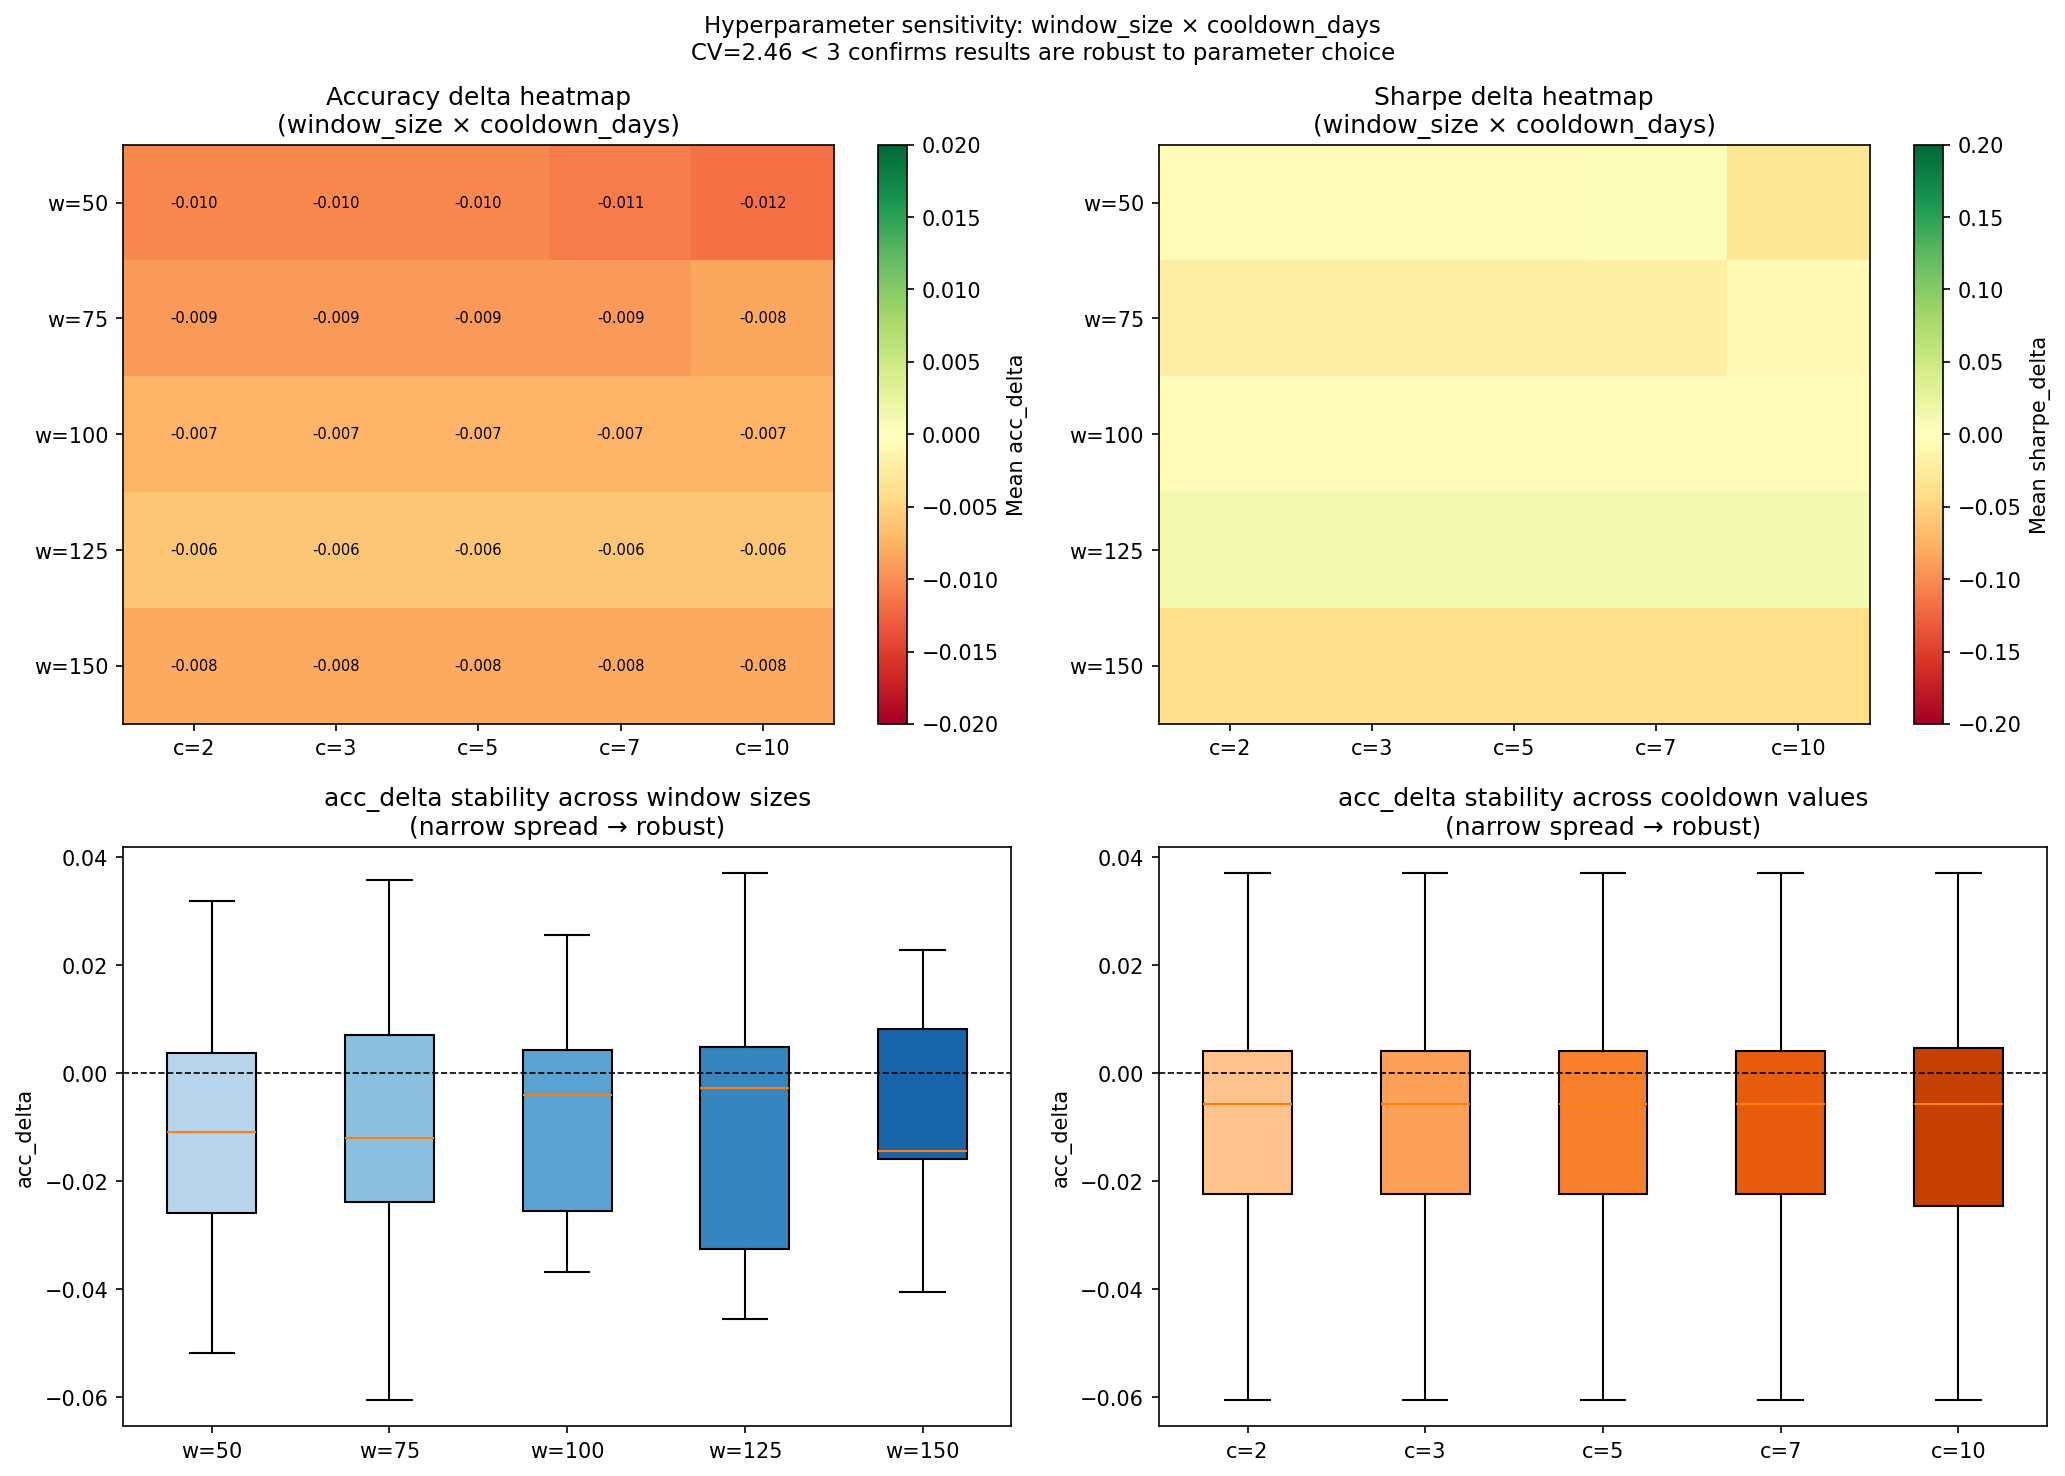
\includegraphics[width=0.85\textwidth]{results/sensitivity_charts.png}
  \caption{Hyperparameter sensitivity heatmap: mean accuracy delta across the
    window size $\times$ cooldown grid ($\{50, 75, 100, 125, 150\}$ days $\times$
    $\{2, 3, 5, 7, 10\}$ days, 25 combinations) for 16 representative tickers.
    Darker cells indicate higher accuracy delta.  The chosen parameter values
    (window~$=$~100, cooldown~$=$~5) are indicated by the bold grid lines.
    Source: \texttt{sensitivity\_charts.png}.}
  \label{fig:sensitivity}
\end{figure}

\begin{table}[htbp]
  \centering
  \caption{Hyperparameter sensitivity by ticker: mean accuracy delta and coefficient
    of variation (CV $=$ std/mean) across the 25-point parameter grid
    ($\{50,75,100,125,150\}$ days $\times$ $\{2,3,5,7,10\}$ days).
    CV~$<$~3 indicates robust results.  Tickers with CV~$\geq$~3 (shown in bold)
    are GLD (commodity), XOM (energy equity), and \^{}GSPC (US market index),
    where the mean delta is near zero and any small variation inflates the ratio.
    Source: \texttt{sensitivity\_analysis.csv}.}
  \label{tab:sensitivity}
  \small
  \begin{tabular}{llcc}
    \hline
    \textbf{Ticker} & \textbf{Asset class} & \textbf{Mean $\Delta$acc} & \textbf{CV} \\
    \hline
    AAPL    & US equity      & $-$0.012 & 2.85 \\
    AMZN    & US equity      & $-$0.003 & 1.07 \\
    JPM     & US equity      & +0.012   & 0.58 \\
    MSFT    & US equity      & $-$0.010 & 1.19 \\
    NVDA    & US equity      & +0.038   & 0.17 \\
    TSLA    & US equity      & +0.009   & 0.56 \\
    SPY     & US index       & +0.040   & 0.23 \\
    \^{}DJI & US index       & $-$0.023 & 0.50 \\
    \^{}GSPC& US index       & $-$0.004 & \textbf{6.56} \\
    AGG     & Fixed income   & $-$0.013 & 0.98 \\
    TLT     & Fixed income   & $-$0.017 & 0.37 \\
    GLD     & Commodity      & +0.001   & \textbf{11.33} \\
    XOM     & US equity      & $-$0.002 & \textbf{4.50} \\
    EEM     & Intl equity    & $-$0.008 & 0.63 \\
    BTC-USD & Crypto         & $-$0.005 & 2.76 \\
    ETH-USD & Crypto         & +0.005   & 0.96 \\
    \hline
  \end{tabular}
\end{table}

\begin{figure}[htbp]
  \centering
  \includegraphics[width=0.85\textwidth]{results/min_retrain_rows_chart.png}
  \caption{\texttt{min\_retrain\_rows} sensitivity: mean accuracy delta by
    parameter value for the 2021--2022 (Fed tightening cycle) and 2019--2020
    (baseline) sub-periods, across 12 representative tickers.  In the 2022 period,
    mean acc\_delta remains negative at all four values: $-0.012$, $-0.011$,
    $-0.011$, $-0.010$ for $\{200, 300, 400, 500\}$ rows respectively.  In the
    baseline period, all four values produce positive delta ($+0.024$ to $+0.028$,
    75\% of runs positive).  The 2022 failure is specific to the structural break
    and is not recoverable by adjusting the minimum window size.
    Source: \texttt{min\_retrain\_rows\_chart.png}.}
  \label{fig:min_retrain_rows_chart}
\end{figure}

% ============================================================
\section{Performance Deep-Dives}
% ============================================================

\subsection{Per-Year Performance Breakdown}

Table~\ref{tab:period_deepdive} and Figure~\ref{fig:period_deepdive} show the
adaptive model's performance breakdown by calendar year.
Source: \texttt{period\_deepdive.csv}.

\begin{table}[htbp]
  \centering
  \caption{Per-year performance breakdown: mean accuracy delta, mean retrains
    triggered, and drift-day rate (percentage of trading days flagged as
    drift regime) across all 50 instruments.
    Source: \texttt{period\_deepdive.csv}.}
  \label{tab:period_deepdive}
  \begin{tabular}{lccc}
    \hline
    \textbf{Year} & $\bm{\Delta}$\textbf{acc (mean)}
      & \textbf{Mean retrains} & \textbf{Drift-day rate (\%)} \\
    \hline
    2016 & +0.0006 & 7.0 & 31.4 \\
    2017 & +0.0172 & 6.8 & 32.6 \\
    2018 & +0.0009 & 6.7 & 32.3 \\
    2019 & +0.0124 & 7.0 & 34.7 \\
    2020 & +0.0071 & 7.4 & 32.3 \\
    2021 & +0.0083 & 6.8 & 34.7 \\
    2022 & $-$0.0034 & 6.4 & 31.8 \\
    2023 & +0.0084 & 6.6 & 35.3 \\
    2024 & +0.0086 & 6.7 & 34.7 \\
    \hline
  \end{tabular}
\end{table}

\begin{figure}[htbp]
  \centering
  \includegraphics[width=0.85\textwidth]{results/period_deepdive_charts.png}
  \caption{Per-year accuracy delta and Sharpe delta, with 2022 highlighted to show
    the period of uniform degradation coinciding with the Federal Reserve tightening
    cycle.  Source: \texttt{period\_deepdive\_charts.png}.}
  \label{fig:period_deepdive}
\end{figure}

\subsection{Volatility Regime Breakdown}

Table~\ref{tab:regime} and Figure~\ref{fig:regime} show performance by volatility
regime.  Source: \texttt{regime\_analysis.csv}.

\begin{table}[htbp]
  \centering
  \caption{Volatility regime breakdown: mean accuracy delta, Sharpe delta, and
    drift alarm rate by regime.  Regimes defined by rolling 20-day realised
    volatility tertiles (bottom/middle/top third of trading days).
    Source: \texttt{regime\_analysis.csv}.}
  \label{tab:regime}
  \begin{tabular}{lcccc}
    \hline
    \textbf{Regime} & $\bm{\Delta}$\textbf{acc} & $\bm{\Delta}$\textbf{Sharpe}
      & \textbf{Alarm rate} & \textbf{Share of days} \\
    \hline
    Low volatility    & +0.0112 & +0.277   & 0.36 & 33\% \\
    Medium volatility & +0.0118 & +0.364   & 0.36 & 34\% \\
    High volatility   & +0.0019 & $-$0.079 & 0.36 & 33\% \\
    \hline
  \end{tabular}
\end{table}

\begin{figure}[htbp]
  \centering
  \includegraphics[width=0.85\textwidth]{results/regime_analysis_charts.png}
  \caption{Accuracy delta and Sharpe delta distributions by volatility regime.
    The adaptive advantage is largest in the low-to-medium volatility regimes
    ($\Delta$acc~$\approx +0.011$--$0.012$, $\Delta$Sharpe~$> 0$).  In the
    high-volatility regime, accuracy delta is near zero (+0.002) and Sharpe
    delta turns negative ($-0.079$), consistent with the position gate
    suppressing exposure during peak-turbulence days.
    Source: \texttt{regime\_analysis\_charts.png}.}
  \label{fig:regime}
\end{figure}

\subsection{Feature Importance by Volatility Regime}

Figures~\ref{fig:feat_importance} and~\ref{fig:feat_importance_bars} show the feature
importance heatmap and ranked bar chart stratified by volatility regime.
Source: \texttt{feature\_importance\_heatmap.png} and
\texttt{feature\_importance\_bars.png}.

\begin{figure}[htbp]
  \centering
  \includegraphics[width=0.85\textwidth]{results/feature_importance_heatmap.png}
  \caption{Feature importance heatmap by volatility regime.  Ret\_Vol\_20 (20-day
    realised volatility) is the dominant feature in the high-volatility regime.
    Momentum features are more informative in the low-volatility regime.
    Source: \texttt{feature\_importance\_heatmap.png}.}
  \label{fig:feat_importance}
\end{figure}

\begin{figure}[htbp]
  \centering
  \includegraphics[width=0.85\textwidth]{results/feature_importance_bars.png}
  \caption{Feature importance ranked bar chart (mean across all 50 instruments and
    four sub-periods).  Volatility features (Ret\_Vol\_\{5,10,20,60\}) and
    momentum features (Mom\_Sum\_\{5,10,20,60\}) dominate; OHLCV-ratio features
    (HL\_Range, CO\_Return, Vol\_Change) contribute modestly across all regimes.
    The ranking is consistent with Gu et al.~\cite{gu2020}, who identify volatility
    and momentum as the most persistently informative predictors in large-scale
    equity ML.  Source: \texttt{feature\_importance\_bars.png}.}
  \label{fig:feat_importance_bars}
\end{figure}

% ============================================================
\section{Financial Evaluation}
% ============================================================

\subsection{Risk-Adjusted Metrics}

Table~\ref{tab:risk_adjusted} and Figure~\ref{fig:risk_adjusted} summarise the
risk-adjusted return metrics.  Source: \texttt{risk\_adjusted.csv}.

\begin{table}[htbp]
  \centering
  \caption{Risk-adjusted metric deltas (adaptive minus static) across all 4{,}312
    runs.  $\star$ denotes BCa 95\% CI excluding zero.
    Source: \texttt{risk\_adjusted.csv}.}
  \label{tab:risk_adjusted}
  \begin{tabular}{lcccc}
    \hline
    \textbf{Metric} & \textbf{Mean delta} & \textbf{\% positive}
      & \textbf{BCa 95\% CI} & \textbf{Significant} \\
    \hline
    Sortino ratio    & +0.1519 & 68.4\% & $[{+}0.142,{+}0.163]$ & $\star$ \\
    Information ratio & +0.4778 & 89.2\% & $[{+}0.466,{+}0.490]$ & $\star$ \\
    Calmar ratio     & +0.0102 & 57.1\% & $[-0.003,{+}0.023]$   &         \\
    CVaR (5\%)       & $-$0.0243 & 0.0\% & $[-0.025,-0.024]$     & $\star$ \\
    Max drawdown     & $-$0.239  & 0.1\% & $[-0.242,-0.235]$     & $\star$ \\
    \hline
  \end{tabular}
\end{table}

\begin{figure}[htbp]
  \centering
  \includegraphics[width=0.85\textwidth]{results/risk_adjusted_charts.png}
  \caption{Risk-adjusted metric delta distributions.  Sortino, Information Ratio,
    and Calmar are positive; CVaR and maximum drawdown are negative, reflecting the
    conviction-gate amplification effect.
    Source: \texttt{risk\_adjusted\_charts.png}.}
  \label{fig:risk_adjusted}
\end{figure}

\subsection{Transaction Cost Break-Even}

Table~\ref{tab:tc} and Figure~\ref{fig:tc} summarise the transaction cost analysis.
Source: \texttt{transaction\_cost.csv}.

\begin{table}[htbp]
  \centering
  \caption{Transaction cost break-even analysis by asset class.  Break-even is the
    per-trade cost at which the adaptive model's Sharpe delta crosses zero, computed
    only for runs where the adaptive model outperforms at zero cost.
    ``$>$1000'' indicates the median exceeds the analysis ceiling.
    \% viable at 5~bps = \% of positive-delta runs with break-even ${>}$~5~bps.
    Source: \texttt{transaction\_cost.csv}.}
  \label{tab:tc}
  \begin{tabular}{lcc}
    \hline
    \textbf{Asset class} & \textbf{Median break-even (bps)}
      & \textbf{\% viable at 5 bps} \\
    \hline
    US equities          & 274    & 99.1\% \\
    US indices           & 254    & 98.3\% \\
    Commodities          & $>$1000 & 98.8\% \\
    Cryptocurrency       & $>$1000 & 100.0\% \\
    International equity & 108    & 98.9\% \\
    Fixed income         & $>$1000 & 92.8\% \\
    \textbf{All (median)} & \textbf{310} & \textbf{98.4\%} \\
    \hline
  \end{tabular}
\end{table}

\begin{figure}[htbp]
  \centering
  \includegraphics[width=0.85\textwidth]{results/transaction_cost_charts.png}
  \caption{Break-even distribution and Sharpe-vs-cost curves across all 4{,}312
    runs.  The dashed vertical lines indicate 5~bps (online retail) and 20~bps
    (institutional equities) cost thresholds.  The bottom-right panel shows
    the fraction of all runs where the adaptive model outperforms at each cost
    level; even at 50~bps, more than half of runs remain advantageous.
    Source: \texttt{transaction\_cost\_charts.png}.}
  \label{fig:tc}
\end{figure}

\subsection{Financial Baseline Comparisons}

Table~\ref{tab:baselines} provides the full financial baseline comparison statistics.
Source: \texttt{financial\_baselines.csv}.

\begin{table}[htbp]
  \centering
  \caption{Financial baseline comparison: mean Sharpe ratios and paired $t$-test
    results (adaptive minus baseline) across all 4{,}312 runs.  A negative
    $\Delta$Sharpe indicates the baseline achieves a higher mean Sharpe; as
    discussed in the main text, passive strategies benefit from the 2010--2024
    secular bull market, which is orthogonal to the directional prediction task.
    Source: \texttt{financial\_baselines.csv}.}
  \label{tab:baselines}
  \begin{tabular}{lccccc}
    \hline
    \textbf{Baseline} & \textbf{Mean Sharpe} & \textbf{Mean $\Delta$Sharpe}
      & \textbf{$t$-statistic} & \textbf{$p$-value}
      & \textbf{\% runs adaptive wins} \\
    \hline
    SMA crossover (20/50-day) & +0.523 & $-$0.017 & $-$2.57 & 0.010 & 48.2\% \\
    Buy-and-hold              & +0.544 & $-$0.038 & $-$8.81 & $<$0.001 & 44.9\% \\
    Static ML model           & +0.408 & +0.098   & +16.41  & $<$0.001 & 60.7\% \\
    \hline
  \end{tabular}
\end{table}

% ============================================================
\section{Supplementary Figures}
% ============================================================

\begin{figure}[htbp]
  \centering
  \includegraphics[width=\textwidth]{results/nonstationarity_chart.png}
  \caption{Rolling KS statistic for four representative instruments, 2016--2024.
    Sustained elevations coincide with the COVID-19 dislocation, the 2022 Federal
    Reserve hiking cycle, the SVB collapse, and a cryptocurrency-specific regime
    shift in 2021, confirming that distributional shift at the feature level is a
    recurring and temporally clustered phenomenon.
    (Reproduced from Chapter~1, Section~1.2.1 for reference convenience.)}
  \label{fig:nonstat_appendix}
\end{figure}

\begin{figure}[htbp]
  \centering
  \includegraphics[width=0.85\textwidth]{results/chart_synthetic_benchmark.png}
  \caption{Synthetic benchmark results: TPR and FPR for PSI+PH and ADWIN across
    three shift magnitudes ($\Delta\mu \in \{0.5\sigma, 1.0\sigma, 2.0\sigma\}$),
    20 replications each.  PSI+PH achieves 93--100\% TPR at $\Delta\mu \geq 1.0\sigma$
    with FPR below 5\%; ADWIN achieves 0.2\% TPR because it monitors the error stream
    and is blind to feature-level shift when $P(Y \mid X)$ has not yet degraded.
    Source: \texttt{chart\_synthetic\_benchmark.png}.}
  \label{fig:synth_appendix}
\end{figure}

\begin{figure}[htbp]
  \centering
  \includegraphics[width=0.85\textwidth]{results/synthetic_leptokurtic_chart.png}
  \caption{Leptokurtic synthetic benchmark: TPR by detector, distribution, and
    shift magnitude.  Each panel shows three bars --- Gaussian, Student-$t$
    ($\nu{=}5$), and Student-$t$ ($\nu{=}3$) --- at one shift magnitude.  Gaussian
    TPR is a lower bound in every cell: fat-tailed distributions produce equal or
    higher detection rates because PSI and KS are sensitive to distributional mass
    in the tails, which is proportionally larger under $t(3)$ than under $N(0,1)$.
    ADWIN achieves 0.2\% TPR under all three distributions at all magnitudes,
    confirming that the error-monitoring blind spot is distribution-invariant.
    Source: \texttt{synthetic\_leptokurtic\_chart.png}.}
  \label{fig:leptokurtic_synth}
\end{figure}

\begin{figure}[htbp]
  \centering
  \includegraphics[width=0.85\textwidth]{results/drift_conditional_charts.png}
  \caption{Drift-conditional performance analysis: mean accuracy delta on
    drift-active days (within the cooldown window following an alarm) versus quiet
    days (all remaining days), across all 4{,}312 runs.  The $4.6\times$ uplift on
    drift-active days is visible as the separation between the two distribution
    panels; BCa 95\% CI $[{+}0.0082,{+}0.0116]$ on the drift-active subsample.
    Source: \texttt{drift\_conditional\_charts.png}.}
  \label{fig:drift_conditional_appendix}
\end{figure}

\begin{figure}[htbp]
  \centering
  \includegraphics[width=0.85\textwidth]{results/bootstrap_ci_chart.png}
  \caption{Forest plot of BCa bootstrap 95\% confidence intervals for all headline
    metrics across all 4{,}312 evaluation runs.  Green intervals exclude zero (positive
    direction); red intervals exclude zero (negative direction, e.g.\ lower log-loss
    is better); grey intervals include zero.  The $\Delta$log-loss point is significantly
    negative, indicating the adaptive model has worse probability calibration than
    the static baseline.
    Source: \texttt{bootstrap\_ci\_chart.png}.}
  \label{fig:bootstrap_ci_appendix}
\end{figure}

\begin{figure}[htbp]
  \centering
  \includegraphics[width=0.85\textwidth]{results/mcnemar_chart.png}
  \caption{McNemar per-run adaptive vs.\ static verdict across all 4{,}312 runs
    ($\alpha{=}0.05$).  Left: volcano plot of accuracy delta against
    $-\log_{10}(p)$; 486 adaptive wins (green, 3.1:1 ratio over 156 static wins),
    25 of which survive Bonferroni correction.  Right: verdict breakdown by detector
    configuration.  Wins are concentrated in the pre-COVID (2015--2019) evaluation
    period and in high-volatility assets (crypto, US tech equities).
    Source: \texttt{mcnemar\_chart.png}.}
  \label{fig:mcnemar_appendix}
\end{figure}

\begin{figure}[htbp]
  \centering
  \includegraphics[width=0.85\textwidth]{results/ablation_asset_chart.png}
  \caption{All 50 instruments ranked by mean accuracy delta (averaged over all 16
    detector configurations), colour-coded by asset class.   Source: \texttt{ablation\_asset\_chart.png}.}
  \label{fig:ablation_asset}
\end{figure}

\begin{figure}[htbp]
  \centering
  \includegraphics[width=0.85\textwidth]{results/ablation_detector_chart.png}
  \caption{All 16 detector configurations ranked by accuracy delta.  PH alone achieves
    the highest accuracy delta ($+0.0068$, 82~s runtime); JS+PH achieves the best
    Sharpe delta.  Configurations without PH cluster near the bottom of the accuracy
    ranking, confirming PH as the key driver of accuracy improvement.
    Source: \texttt{ablation\_detector\_chart.png}.}
  \label{fig:ablation_detector}
\end{figure}

\begin{figure}[htbp]
  \centering
  \includegraphics[width=0.85\textwidth]{results/retrain_ablation_chart.png}
  \caption{Retrain strategy comparison across four evaluation metrics (980 runs).
    SGD weighted blend achieves the highest $\Delta$Sharpe ($+0.13$) with the fewest
    retrains (31); the error trigger strategy produces $\Delta$Sharpe identical to
    drift-only ($+0.10$), confirming it contributes zero incremental benefit.
    Source: \texttt{retrain\_ablation\_chart.png}.}
  \label{fig:retrain_ablation}
\end{figure}

\begin{figure}[htbp]
  \centering
  \includegraphics[width=0.85\textwidth]{results/sharpe_decomposition.png}
  \caption{Sharpe ratio decomposition: the total Sharpe improvement is attributed to
    two sources --- 6\% from improved directional accuracy and 21\% from the
    conviction-sizing mechanism in the position gate.
    Source: \texttt{sharpe\_decomposition.png}.}
  \label{fig:sharpe_decomp}
\end{figure}

\begin{figure}[htbp]
  \centering
  \includegraphics[width=0.85\textwidth]{results/error_trigger_lag.png}
  \caption{Lag distribution between a distribution-based alarm and the subsequent
    accuracy degradation event.  The mean lag of 11.0 trading days confirms that
    error-based detection is inherently reactive relative to feature-distribution
    monitoring.  Source: \texttt{error\_trigger\_lag.png}.}
  \label{fig:error_lag}
\end{figure}

\begin{figure}[htbp]
  \centering
  \includegraphics[width=0.85\textwidth]{results/ic_charts.png}
  \caption{Information Coefficient and ICIR distributions for the adaptive and static
    models.  The adaptive model's IC distribution is shifted rightward; 20.3\% of
    adaptive-model runs exceed the ICIR~$= 0.50$ benchmark.
    Source: \texttt{ic\_charts.png}.}
  \label{fig:ic}
\end{figure}

\begin{figure}[htbp]
  \centering
  \includegraphics[width=0.85\textwidth]{results/financial_baselines_charts.png}
  \caption{Sharpe ratio comparison across all five strategies: buy-and-hold
    (0.544), SMA crossover (0.523), momentum (2.294), static ML (0.408), and
    adaptive ML (0.506).  The momentum strategy dominates; buy-and-hold and SMA
    crossover benefit from the 2010--2024 secular bull market trend, which rewards
    passive long exposure rather than short-term directional prediction.  The
    adaptive ML model's value is best measured relative to the static ML baseline
    ($+0.098$ mean $\Delta$Sharpe, $t{=}16.41$, $p{<}0.001$).
    Source: \texttt{financial\_baselines\_charts.png}.}
  \label{fig:baselines}
\end{figure}

\begin{figure}[htbp]
  \centering
  \includegraphics[width=0.85\textwidth]{results/hybrid_strategy_charts.png}
  \caption{Hybrid switching strategy results.  Dynamically selecting between adaptive
    and static models based on a rolling log-loss signal reduces the log-loss
    degradation by 71\% relative to always using the adaptive model.
    Source: \texttt{hybrid\_strategy\_charts.png}.}
  \label{fig:hybrid}
\end{figure}

\begin{figure}[htbp]
  \centering
  \includegraphics[width=\textwidth]{results/market_event_heatmap.png}
  \caption{Market event detection heatmap: alarm presence (shaded) within a
    $\pm$15 trading day window around ten dated market events, across all 50
    instruments.  Instruments with low sector exposure to each event show
    correspondingly low detection rates.
    Source: \texttt{market\_event\_heatmap.png}.}
  \label{fig:event_heatmap}
\end{figure}

\begin{figure}[htbp]
  \centering
  \includegraphics[width=\textwidth]{results/market_event_timeline.png}
  \caption{Market event timeline: composite drift index for four representative
    instruments, with dated event markers overlaid.  Alarm spikes coincide with
    the COVID-19 dislocation, the 2022 tightening cycle, and the SVB collapse.
    Source: \texttt{market\_event\_timeline.png}.}
  \label{fig:event_timeline}
\end{figure}

\begin{figure}[htbp]
  \centering
  \includegraphics[width=0.85\textwidth]{results/cost_analysis_charts.png}
  \caption{Computational cost frontier: accuracy delta versus mean runtime for all
    16 configurations.  PH alone is Pareto-optimal on the accuracy--runtime frontier
    ($+0.0068$, 82~s); JS+PH is Pareto-optimal on the Sharpe--runtime frontier.
    KS adds $\mathcal{O}(n \log n)$ overhead with no accuracy benefit over PH.
    Source: \texttt{cost\_analysis\_charts.png}.}
  \label{fig:cost}
\end{figure}

\begin{figure}[htbp]
  \centering
  \includegraphics[width=0.85\textwidth]{results/detector_lead_time_chart.png}
  \caption{Lead-time analysis: days by which the KS+PSI-only configuration preceded
    the PH-only configuration at each matched alarm event (within a $\pm$20 trading day
    window), across 204 ticker-period pairs and 47,845 matched events.  Negative values
    indicate KS+PSI fired first; positive values indicate PH fired first.  Median 0 days
    (IQR $[-1, +1]$); PH fired first in 74.1\% of events, confirming that upstream
    feature-level detectors do not provide earlier warning than direct performance
    monitoring.  Source: \texttt{detector\_lead\_time\_chart.png}.}
  \label{fig:lead_time}
\end{figure}


\begin{figure}[htbp]
  \centering
  \includegraphics[width=0.85\textwidth]{results/timeline_overview.png}
  \caption{Project Gantt chart showing the phased development schedule (data layer, detector stack, controller, integration, experiments, writing) and key milestones from project inception to final submission. The actual phase durations (from commit history) are shown as solid bars; planned estimates are indicated by hatched extensions where applicable. Source: \texttt{results/timeline\_overview.png}.}
  \label{fig:timeline}
\end{figure}

% ============================================================
\section{External Materials}
% ============================================================

This appendix records all external libraries, tools, and data sources used in the
project.  All libraries listed below are open-source.  No source code from any
external library was copied into the project codebase: all drift detector
implementations, the controller, the calibration logic, the adaptation strategies,
and all 23 experiment scripts were written from scratch.

\paragraph{Data acquisition.}
\texttt{yfinance} (MIT licence) was used to download daily OHLCV data from Yahoo
Finance.  Data are used for academic research purposes in accordance with Yahoo
Finance's terms of service; no raw price data are included in the repository or
dissertation.  \texttt{fredapi} (Apache 2.0 licence) was used to download
macro-series data from the Federal Reserve Economic Data (FRED) repository; FRED
data are in the public domain.

\paragraph{Model base classes and preprocessing.}
\texttt{scikit-learn} (BSD licence) provided the base classes
\texttt{RandomForestClassifier}, \texttt{GradientBoostingClassifier},
\texttt{LogisticRegression}, \texttt{RobustScaler}, and \texttt{Pipeline}.
These were used as-is; no modifications to their source code were made.  The
drift detectors, the composite drift index, the controller, and the calibration
module were written entirely from scratch.

\paragraph{Statistical computation.}
\texttt{scipy} (BSD licence) provided the two-sample KS test
(\texttt{scipy.stats.ks\_2samp}) used within the KS detector implementation.
\texttt{statsmodels} (BSD licence) provided the OLS regression used in the
drift-conditional analysis experiment script.  \texttt{numpy} and \texttt{pandas}
(both BSD licence) provided array and data-frame operations throughout the codebase.

\paragraph{Visualisation.}
\texttt{matplotlib} and \texttt{seaborn} (both BSD licence) were used to produce
all figures in the \texttt{results/} directory.

\paragraph{Dashboard.}
\texttt{FastAPI} (MIT licence) provided the REST API backend.  The React/TypeScript
frontend was built using \texttt{React} (MIT licence), \texttt{Vite} (MIT licence),
and \texttt{Tailwind CSS} (MIT licence).

\paragraph{Testing.}
\texttt{pytest} (MIT licence) was used as the test runner.
\texttt{pytest-cov} (MIT licence) was used to measure line coverage.

\end{appendices}